%!TEX root = ../../thesis.tex
%=============================================================================


\section{Dataset Evaluation}
\label{eval:dataset}

In this section, an evaluation of the proposed pipeline and an existing solution on a pre-existing data set will be presented.
The goal of this evaluation is to take a closer look at the performance of the proposed pipeline with the explicit focus on computational cost as well as time needed for recognizing speech.

Based on the additional features the proposed pipeline introduces, most prominently synchronization of speech results and the modular nature of the pipeline (see chapters TODO), we expect the proposed pipeline to consume more CPU power as well as taking longer to compute results in comparison to the existing solution.
To further examine the cost, we will in particular inspect the cost different additional components will add to the pipeline to determine the scaling of the proposed pipeline.

We will lastly discuss if this additional cost renders the pipeline unsuitable for real world applications or if the benefits outweigh these costs.


\subsection{Tested Pipeline Configurations}

\subsubsection{Existing Solution}

The existing solution only consists of the \gls{psa}, see figure \ref{pic:eval_p1_diag}.
The \gls{psa} grabs audio from a microphone using ALSA, filters the audio using an integrated voice activity detection and finally uses, as its name suggests, \gls{ps} to recognize speech.
Results are then published via ROS.

The \gls{psa} was and is used extensively for several years in the RoboCup@Home setup of Team ToBi \cite{ToBi}.
In this evaluation it is primarily used to provide a baseline for the proposed pipeline and context for the acquired results.

\begin{figure}[]
	\centering
	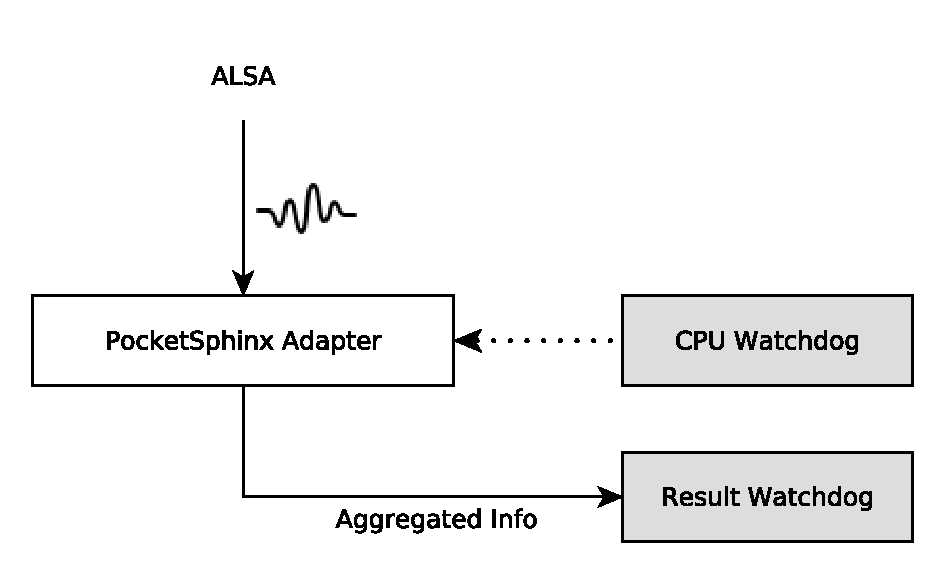
\includegraphics[width=0.66\textwidth]{diagrams/eval_pipeline_1.pdf}
	\caption{Test scenario for existing pipeline.
		The \gls{psa} acquires audio data from ALSA and provides speech recognitions.
		A CPU and result watchdog monitor and log its CPU usage and results respectively.}
	\label{pic:eval_p1_diag}
\end{figure}

\subsubsection{Baseline for proposed Pipeline}
\label{eval:dataset:pipeline:baseline}
This configuration of the proposed pipeline is intended to reassemble the \gls{psa} as closely as possible.
As seen in figure \ref{pic:eval_p2_diag}, it consists of a voice activity detection, a speech recognizer (using \gls{ps}), the Orchestrator and a Wav file player to feed audio into the pipeline.
Recognition results are gathered by the Orchestrator and then communicated via ROS.

\begin{figure}[]
	\centering
	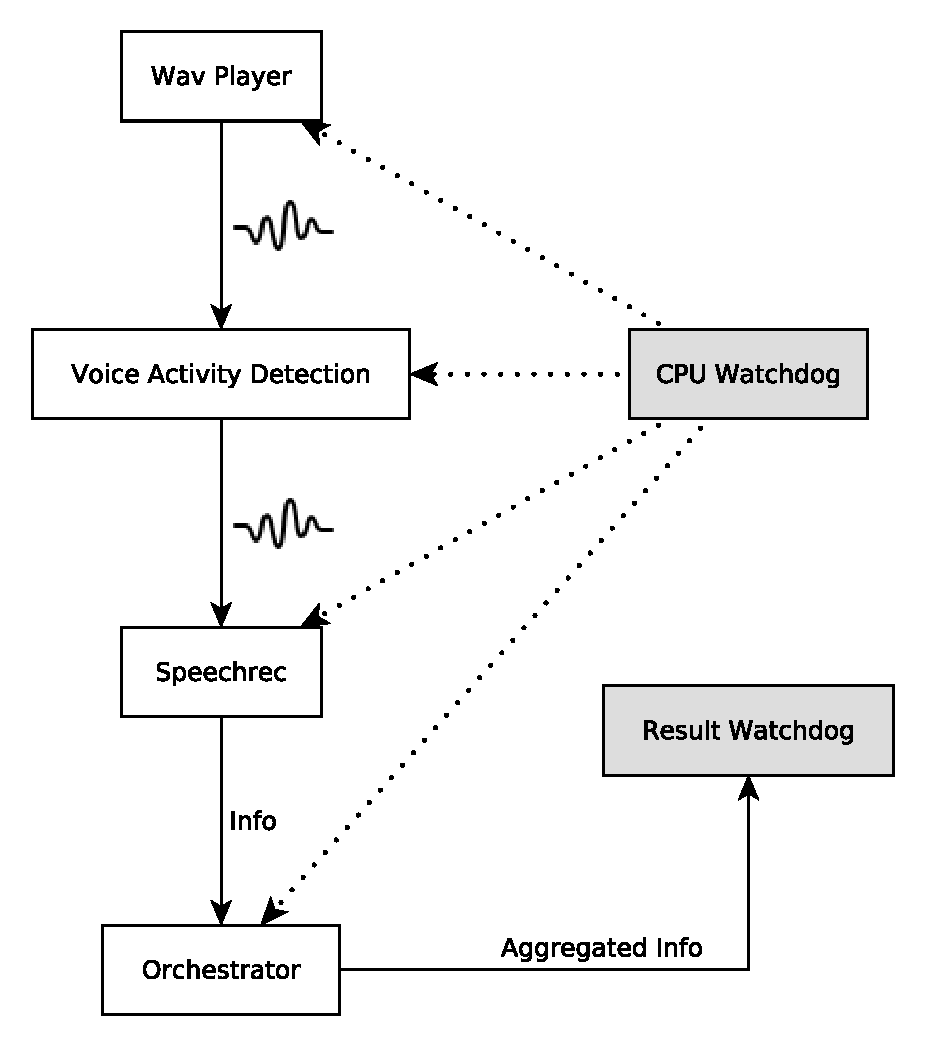
\includegraphics[width=0.66\textwidth]{diagrams/eval_pipeline_2.pdf}
	\caption{Test scenario for proposed pipelines baseline.
		It consists of a wav player, which provides audio data.
		The audio is then processed by a \gls{vad} and a speech recognizer.
		The Orchestrator gathers the speech recognizers data and provides it to a result watchdog, which then saves the results.
		A CPU watchdog monitors and logs CPU usage of all components.}
	\label{pic:eval_p2_diag}
\end{figure}


\subsubsection{Elongated baseline of proposed Pipeline}
This configuration of the proposed pipeline is nearly identical to its baseline, but incorporates a dummy component to evaluate how much overhead in time and CPU cost an additional processing step produces.
As indicated in figure \ref{pic:eval_p4_diag} and by its name, the dummy node does neither alter nor compute information on the audio data it receives, but instead just relays it from the WAV player to the \gls{vad}.

\begin{figure}[]
	\centering
	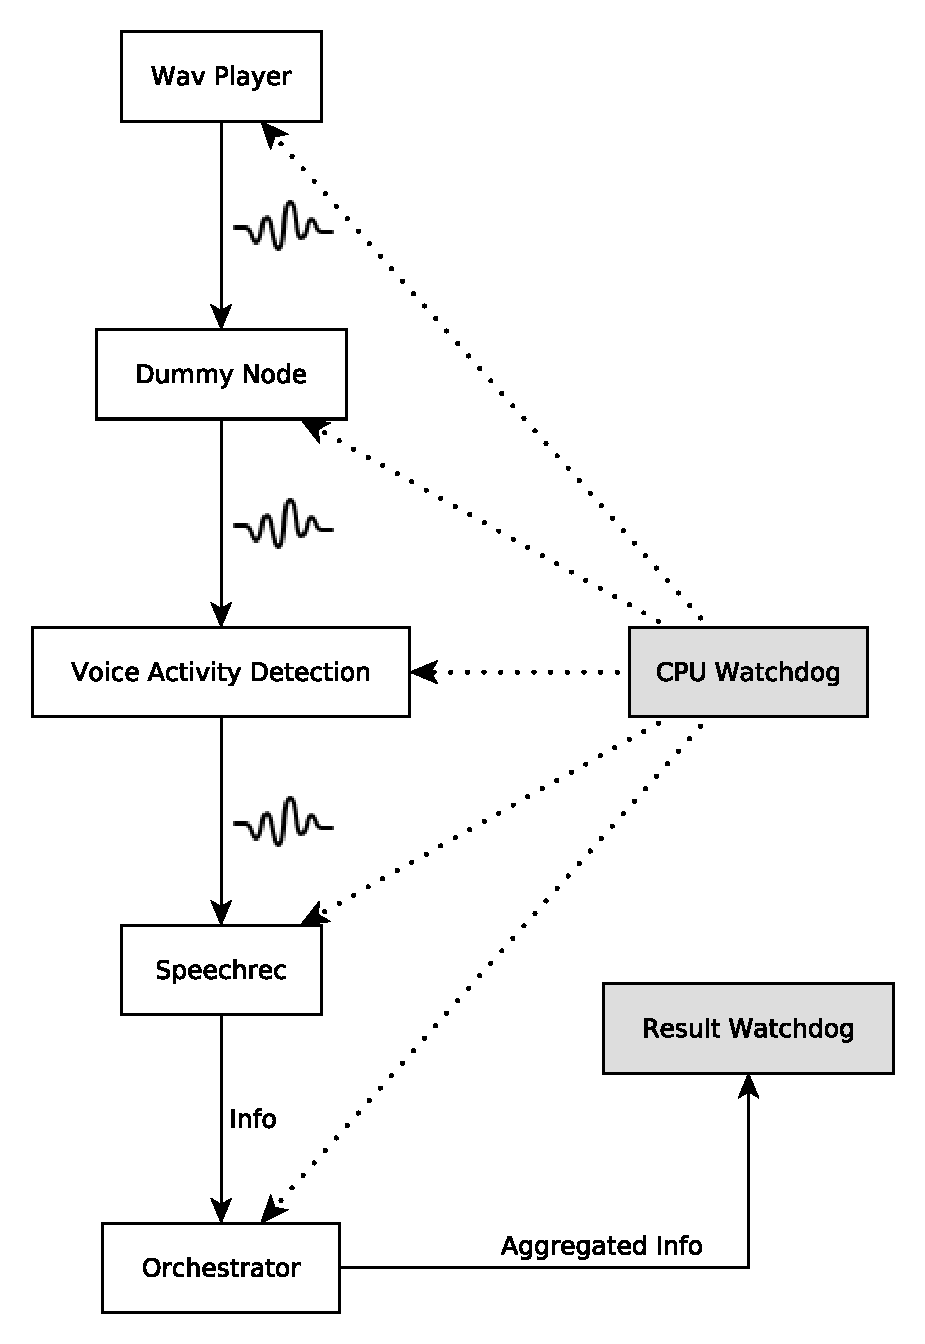
\includegraphics[width=0.66\textwidth]{diagrams/eval_pipeline_4.pdf}
	\caption{Test scenario for an elongated configuration of the proposed pipeline.
		In comparison to the baseline of the proposed pipeline, it encompasses an additional dummy node which is squeezed in between the wav player and the \gls{vad}.
		It does not alter the audio in any way, but is monitored by the CPU watchdog as well.}
	\label{pic:eval_p4_diag}
\end{figure}

\subsubsection{Widened baseline of proposed Pipeline}
This configuration of the proposed pipeline is nearly identical to its baseline, but incorporates a dummy component to evaluate how much overhead in time and CPU cost an additional information provider produces.
As indicated in figure \ref{pic:eval_p3_diag} and by its name, the dummy node receives audio data from the \gls{vad} and works basically in parallel to the speech recognizer.
Upon receiving audio data, the dummy node provides hard coded information to the Orchestrator.
This way the Orchestrator does not have to wait on receiving the dummy nodes information during its synchronization steps, and can theoretically provide synchronized data as soon as speech recognition results are provided to it.

\begin{figure}[]
	\centering
	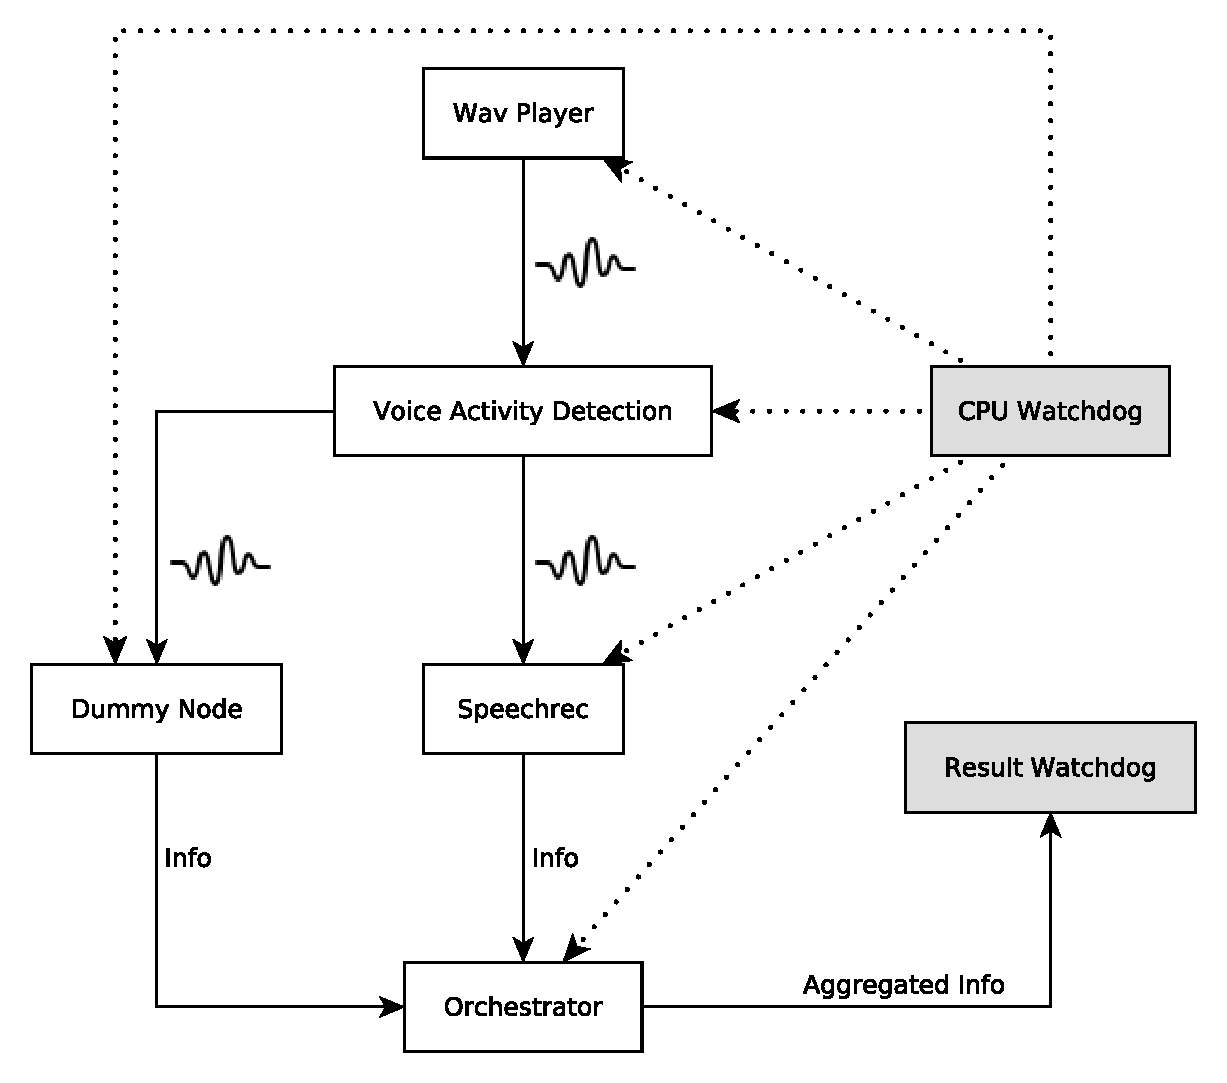
\includegraphics[width=0.66\textwidth]{diagrams/eval_pipeline_3.pdf}
	\caption{Test scenario for an widened configuration of the proposed pipeline.
		In comparison to the baseline of the proposed pipeline, it encompasses an additional dummy node which is set in parallel to the speech recognizer and provides hard coded information to the Orchestrator, which then synchronizes these information with those it received from the speech recognizer.}
	\label{pic:eval_p3_diag}
\end{figure}


\subsubsection{Realistic version of proposed Pipeline}
This configuration of the proposed pipeline resembles its baseline, but includes two additional information provider. 
One provides information on the gender of the speaking person while the other provides information about their emotional status.
As shown in figure \ref{pic:eval_p5_diag}, both additional components run in parallel to the speech recognition and provide the Orchestrator with their information.

This configuration of the pipeline is intended to resemble a realistic use case of the proposed pipeline, in that several speech information need to be synchronized.

\begin{figure}[]
	\centering
	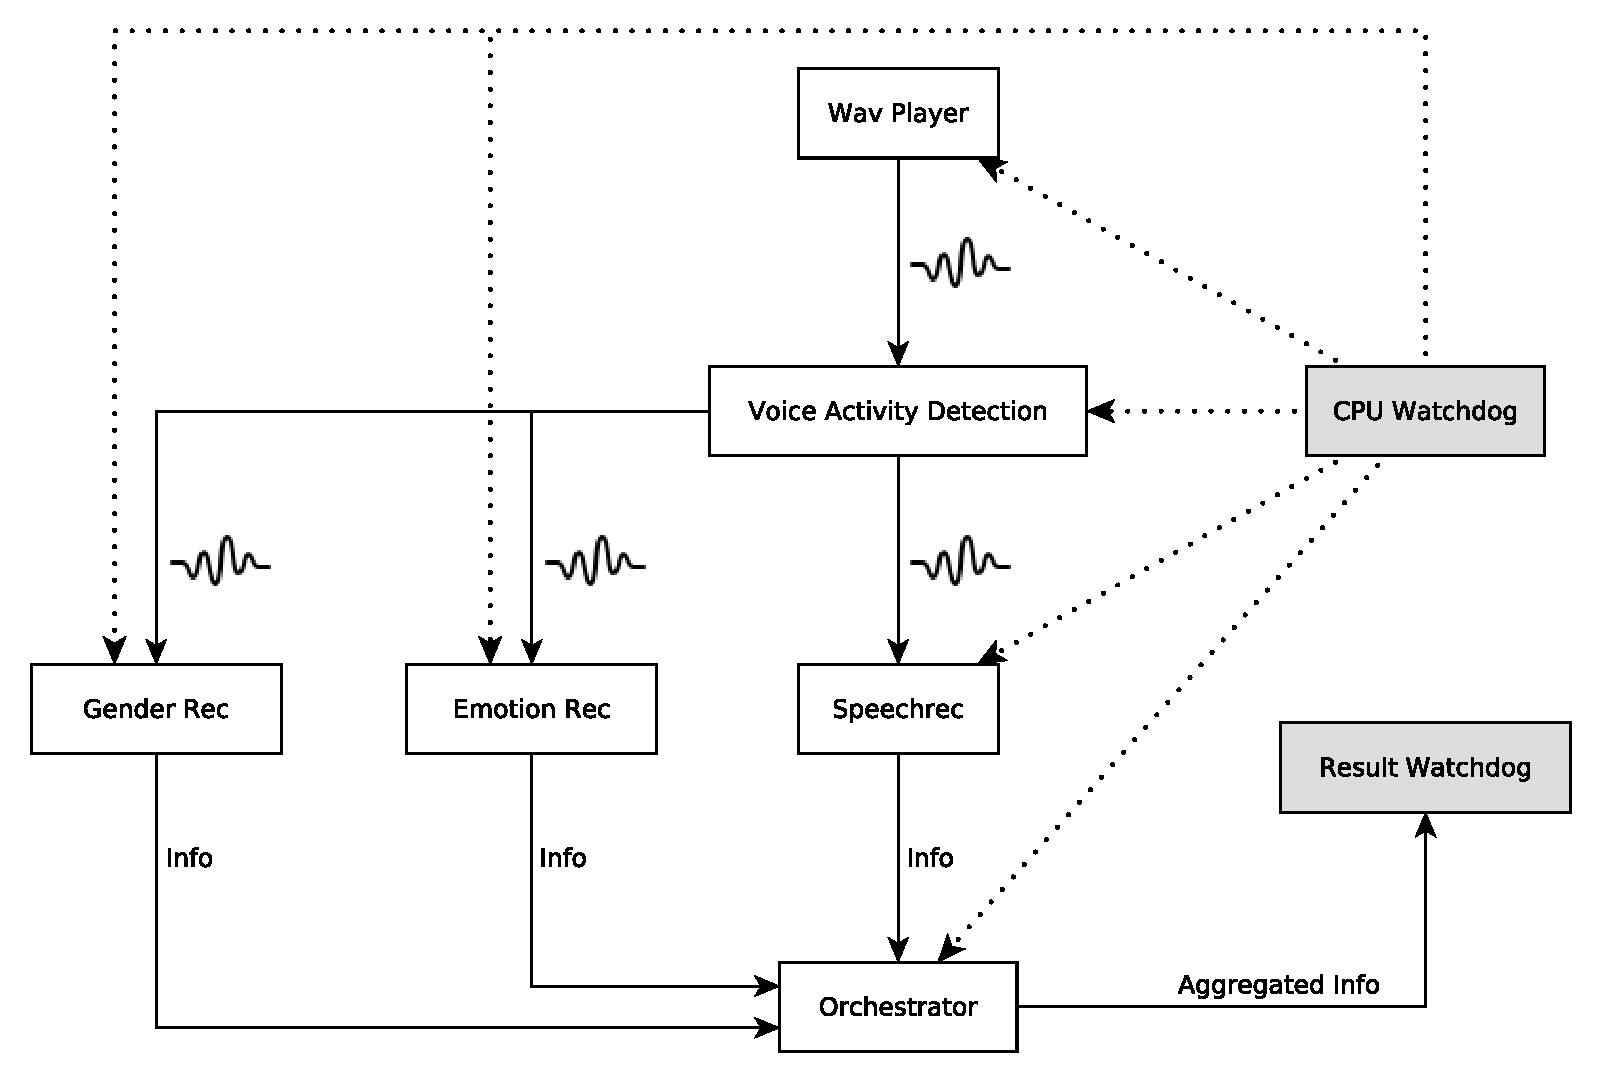
\includegraphics[width=0.66\textwidth]{diagrams/eval_pipeline_5.pdf}
	\caption{Test scenario for an realistic configuration of the proposed pipeline.
		In comparison to the baseline of the proposed pipeline, it encompasses two additional components which are set in parallel to the speech recognizer, namely a gender and a emotion recognizer.
		Both provide additional information to the Orchestrator, which then synchronizes these information with those it received from the speech recognizer.}
	\label{pic:eval_p5_diag}
\end{figure}

\subsubsection{Dataset}
\label{eval:dataset:dataset}

The data set (see figure \ref{table:eval_dataset_info}) used for this evaluation consists of 1723 samples ranging between a half and fourteen seconds.
It incorporates twelve speakers (male and female) speaking 24 phrases. 
Individual samples were recorded using two microphones, one omni directional and one cardioid.
They were recorded in two rooms, some of them with noise, others without.

To more easily feed all samples into the existing solution, the wav files containing the samples were concatenated into one big wav file, with three seconds of silence added in between the individual samples, to easily distinguish the samples from one another.
This also simplifies matching the recorded speech recognition results with the actual utterances.
The proposed pipeline was fed each sample individually, but three seconds of silence were similarly inserted into the audio.

The complete data sets playtime including the silence amounted to nearly two hours and fifty minutes.


\begin{figure}[]
	\centering
	\begin{tabular}{| l | r |}
		\hline
		Samples 				& 1723	 	\\ \hline
		Phrases	in kitchen		& 1149		\\ \hline
		Phrases	in wardrobe		& 574		\\ \hline
		Noisy Phrases			& 575		\\ \hline
		Clean Phrases			& 1148		\\ \hline
		Individual Phrases		& 24 		\\ \hline
		Speakers 				& 12	 	\\ \hline
		Female					& 5 		\\ \hline
		Male	 				& 7			\\ \hline
		Runtime (w/ silence) 	& 2:49:23	\\ \hline
		Runtime (w/o silence) 	& 1:23:01	\\ \hline
		Language 				& German	\\ \hline
	\end{tabular}
	\caption{Detailed Information about the Data Set.}
	\label{table:eval_dataset_info}
\end{figure}

\subsubsection{Setup}
\label{eval:dataset:setup}

Two slightly different setups were used for the various configurations of the proposed pipeline on the one hand and the existing solution on the other, due to differences in acquiring audio data.
What they have in common is that all pipelines were tested on the same computer, a Thinkpad Carbon X1 Gen with a Intel(R) Core(TM) i7-7500U, to ensure equal CPU performance.

All setups were comprised of equivalent components. 
If not otherwise stated, all variations of the proposed pipeline used the exact same components with identical configurations (safe for some minor details, e.g. a modified path for the audio between the wav player, dummy node and \gls{vad} in the elongated version of the proposed pipeline, see figure \ref{pic:eval_p2_diag} and \ref{pic:eval_p4_diag}).

The existing pipeline's \gls{psa} internally incorporates a \gls{vad}, which was reimplemented and used as the \gls{vad} of the proposed pipelines.
It uses \gls{ps} for speech recognition, as does the speech recognizer used in the proposed pipeline. 
Both \gls{ps} instances use the same speech models, dictionary, and grammar.

In both cases two small scripts were used to record the components CPU usage as well as speech recognition results and timings.
CPU usage was universally recorded using the python library psutil \cite{psutil} and its cpu\_times functionality.
However, psutils reliability can be called into question, as it seems to not take modern CPU's capabilty to increase or decrease their clock speed, denpending on load, into account.
As such, the recorded CPU costs should rather be taken as rough estimates and not as exact measurements.
Nonetheless, we included these data points despite their supposed inaccuracy because apart from one tested pipeline, all pipelines did not produce enough load on the CPU to cause it to increase its clock speed.
This is supported by the fact that identical components across various pipelines produce very similar CPU loads, as seen in figure 
\ref{table:eval_dataset_detail}.
Incidentally, a process producing the computational load of one CPU second over any timespan is equal to the process running on one core of a CPU under full load for one second.

Speech recognition results were recorded by a ROS node which collected ROS messages published by the proposed pipeline's orchestrator and the \gls{psa} respectively.

\subsubsection{Recording Results}

The times needed to calculate results were recorded in two different ways.
Due to the fact that the proposed pipeline annotates its results with the time the audio was recorded, it is rather simple to calculate the time needed for recognition.
One can simply subtract the time when the analyzed audio signal ended from the time the synchronized result was received by the recording component and thus, get the total time needed for recognition.
To be precise, this way we measure the time from when the segmentation ends to the point where the recording node received the recognized speech result.

The method of feeding audio into the proposed pipeline does not matter as long as the timestamps of the audio are correct.
So instead of grabbing the audio via a microphone we used a wav-file player to feed the data set directly into the pipeline.

The existing solution however was in need of a small workaround to work on audio files rather than audio directly grabbed by a real microphone.
A virtual microphone was needed to feed the data set into the \gls{psa}.
This virtual microphone provided access to a wav file containing the data set. 
As information about singular utterances inside the data set could not be propagated through ALSA and the \gls{psa}, we recorded a timestamp with the start of feeding the wav file into the virtual microphone and thus in turn into the \gls{psa}.
Speech recognition results were then recorded along timestamps acquired when these results were received in the dedicated ROS node.
Supplementary, while concatenating the data set into the singular wav file, we created annotations to keep track of when each sample ended and which phrase it contained.
To achieve comparable results, slight modifications to the internal segmenter of the \gls{psa} were made, i.e. timestamps on each successful segmentation would be recorded.

By combining the information provided by these annotations, the timestamp created during the start of feeding the wav file, the timestamps recorded when recording the speech recognition results and after each successful segmentation, the absolute time needed by this solution could be computed. 
This is mostly done by subtracting the timestamp collected after a successful segmentation from the corresponding recorded when the results were received. TODO
Thus, we record the time from the segmentations end to receiving the results, as previously with the proposed pipeline.

In any case, speech recognition results and timings were recorded as raw data and written to files.
Afterwards, these raw results could be processed and evaluated with the help of further scripts.

\begin{figure}[]
	\centering
	\begin{tabular}{ | l | p{0.2\textwidth} | p{0.2\textwidth} | r|}
		\hline
		Pipeline 	& Recognition percentage & Absolute time till result & Sum CPU time \\ \hline
		Existing 	& 77.02\% & 0.063 sec &   228.99 sec \\ \hline
		Proposed 	& 99.77\% & 1.014 sec &  1209.30 sec \\ \hline
		Elongated 	& 99.77\% & 1.039 sec &  1399.63 sec \\ \hline
		Widened 	& 99.65\% & 1.090 sec &  1665.66 sec \\ \hline
		Realistic 	& 99.48\% & 1.780 sec & 37517.13 sec \\ \hline
	\end{tabular}
	\caption{Results of the different pipelines in comparison.
		Shown are percentage of correct recognition, average time for recognition and consumed CPU time.}
	\label{table:eval_dataset_results}
\end{figure}

\begin{figure}[]
	\centering
	\begin{tabular}{ | l | r | r | r | r | r |}
		\hline
		Component 	& Existing 	& Proposed & Elongated & Widened & Realistic\\ \hline
		Speech Rec 	& 247.44 	& 546.65 & 545.73 & 574.82	 &   285.77 \\ \hline
		Orchestrator& - 		& 107.66 & 114.69 & 415.73	 &   962.56 \\ \hline
		Wav Player 	& -			& 380.11 & 378.71 & 405.40	 &   138.22 \\ \hline
		\gls{vad}		 	& - 		& 174.88 & 188.56 & 191.97	 &    51.26 \\ \hline
		Dummy	 	& - 		& -		 & 171.94 &  77.74	 &        - \\ \hline
		Gender Rec 	& - 		& -		 & -	  & -	 	 &  5959.50 \\ \hline
		Emotion Rec	& - 		& -		 & - 	  & -		 & 30119.82 \\ \hline
	\end{tabular}
	\caption{Detailed CPU cost by pipeline and component.
		}
	\label{table:eval_dataset_detail}
\end{figure}

\subsection{Discussion}
\label{eval:discussion}

% Pipeline 1 & 2 ----------------------------------------------------------

{ % 10 
If one compares the recognition percentages of all the pipelines in figure \ref{table:eval_dataset_results}, the various configurations of the proposed pipeline all share virtually identical results, which however differs significantly from the \gls{psa}'s result.
This is somewhat unexpected, as special care was taken to ensure both speech recognizers use not only \gls{ps}, but also equal configuration files, including speech model, dictionary and grammar.
As the audio segmentation for the proposed pipeline is a reimplementation of the one used internally in the \gls{psa}, and was furthermore basically bypassed in that the silence in between samples enabled the usage of very lenient \gls{vad} configurations.

The proposed pipelines \gls{ps} component is written in Python and uses its \gls{ps} wrapper, which in turn makes use of the same C++ libraries as the \gls{psa}, so it would be difficult to claim this as the determining difference responsible for this discrepancy.
Clearly more testing is needed to produce substantiated suppositions about the difference in recognition results.
}

% pipeline 4

{ % 20
If one compares the results of the proposed and elongated pipeline in figure \ref{table:eval_dataset_results}, a slight increase in absolute time per recognition can be seen, as well as a moderate increase in CPU cost.
The increase in CPU cost is virtually completely due to the additional dummy component present in this pipeline, as can be extracted from figure \ref{table:eval_dataset_detail}. 

The slight increase of 15ms in absolute recognition time was, as discussed before, expected.
Considering a very elaborate configuration, where audio would be transmitted through audio grabbing, sound source localization, beamforming, audio enhancement, \gls{vad} and speech recognition, the latency introduced by using the proposed pipeline could be estimated to have an upper bound of 90ms.
This would barely be humanly noticeable and depending on the time taken by the components themselves probably be just a fraction of the absolute recognition time needed.
%Considering the \gls{vad}, which utilizes a computationally very inexpensive algorithm to segment the audio and should introduce only a slightly larger latency into the pipeline.
}

% pipeline 3
{ % 30
The widened configuration of the proposed pipeline is the first discussed configuration in which the Orchestrator has to actually synchronize data. 
In the baseline and elongated configuration it could take advantage of not having any other information provider and just relay all incoming data.
The additional computational power required by the Orchestrator can easily be observed in figure \ref{table:eval_dataset_detail}.
Though, this configuration of the pipeline seems to generally have higher computational load, probably due to reasons discussed in section \ref{eval:dataset:setup}.
The Orchestrator is responsible for around a quarter of the computational load of the whole pipeline compared to roughly a tenth in the baseline and elongated configuration.

The moderate uptick in absolute recognition time may also be explained by the additional synchronization work the Orchestrator has to contribute. 
This increase of 86ms in itself should not be particularly noticeable as it increases the absolute recognition time by just around 8 percent, which could be seen as a valuable trade-off for gaining synchronized speech results. 
However, further tests could be carried out to investigate the scaling of this particular part of the proposed pipeline.
}

% pipeline 5
{ % 40
Regarding the realistic pipeline the absolute time for recognition saw a significant increase in comparison to the baseline of the proposed pipeline, as can be seen in figure \ref{table:eval_dataset_results}.
Thanks to the Orchestrator saving all received information inside its database, as described in chapter TODO, it was possible to inspect the latencies of each component individually.
The emotion and gender recognizers latency proved to be three and thirteen times as large as the speech recognizers, which can be supported by inspecting their CPU cost in figure \ref{table:eval_dataset_detail}.
This leads to the assumption that the defining factor for the increase in time needed for recognition is actually the result of these components needing more time to compute their results.
As this is a expected feature of the proposed pipeline, the longer time for recognition is a trade-off for having synchronized results.
}
% old stuff

{ % 50
The baseline of the proposed pipeline consuming at least six times as much CPU power as the existing solution, as can be seen in figure \ref{table:eval_dataset_results} may seem like an tremendous increase.
But in comparison to the playtime of nearly 2 hours and 50 minutes the CPU time cost of circa 20 minutes and 4 minutes for the proposed pipeline and the existing solution respectively are both more than acceptable, especially considering that most modern CPUs have more than one core and this load is shared between them.

Additionally, we should keep in mind that \gls{ps} was designed years ago to work on mobile devices of that time, so it is one of the computational most inexpensive speech recognizers still used. 
Despite this it is the computationally most demanding component of all the proposed pipelines configurations apart from the realistic one.

More modern speech recognizers can generally be divided into offline and cloud services.
Cloud based speech recognizers, such as Google \cite{GoogleSpeech} or Microsoft \cite{MicrosoftSpeech} speech to text services produce varying degrees of latency, as audio must first be streamed to distant datacenters before it can be processed and the results can be sent back.
Depending on the available internet connection and the time spend analyzing the audio, these approaches typically take at least as long as fast offline approaches.

Modern offline approaches mostly focus on deep learning at the time of writing. %TODO: citation needed
As such they often use elaborate neural networks which can only be run on graphics cards in a timely manner and are computationally exceptionally costly.

The results of the realistic version of the proposed pipeline reflect this.
Both the gender and emotion recognizer used in the pipeline use rather simple, but nevertheless computationally costly neural networks.
Still, they exceed the cost of all other pipelines by more than a factor of 20.

Based on this and the fact that all components of the proposed pipeline can easily be swapped out, the actual resource cost the components themselves introduce may not even matter that much, as each component could easily be replaced, either by one performing better but being less resource efficient or vice versa.
}


{ % 60
As can clearly be seen in figure \ref{table:eval_dataset_results}, each configuration of the proposed pipeline takes over a second to compute speech recognition results, which seems extremely high in comparison to the existing solution.
Considering the insights procured with the elongated version of the proposed pipeline, recognition time should in the presented configurations never increase by over 100ms due to audio transferring.

The argument could be made that due to the recognition results being different between the \gls{psa} and proposed pipelines' \gls{ps}, both implementations could behave fundamentally different from one another.
This could explain the proposed pipelines \gls{ps} component to perform better while also consuming considerably more CPU time.
But even when scaling the \gls{psa}'s recognition time to match the six times higher CPU cost of the proposed pipeline, the \gls{ps} component's part of the recognition time would only amount to around 320ms.

In a worst case scenario, summing up these upper bounds on added recognition time would result in an average time of about 420ms.  
Due to the actually measured time being more than twice that, we suspect some sort of bug to be responsible for this behavior, which sadly could not be eliminated because of time constraints and would be material for future work.

Regardless, as the results of the widened and elongated configurations of the proposed pipeline indicate, this bug appears to only add a fixed amount of time needed for recognition and not to scale with the number of its components. 
}





